\documentclass[11pt,a4paper]{article}
\usepackage[T1]{fontenc}
\usepackage{lmodern,microtype}
\usepackage{amsmath,amssymb,amsthm,mathtools}
\usepackage{geometry,booktabs,array,enumitem}
\usepackage[colorlinks=true,linkcolor=blue,urlcolor=blue,citecolor=blue]{hyperref}
\usepackage{tikz}
\geometry{margin=25mm}
\setlist[itemize]{leftmargin=1.8em}
\newtheorem{theorem}{Theorem}
\newtheorem{lemma}[theorem]{Lemma}
\newtheorem{proposition}[theorem]{Proposition}
\newcommand{\Rstar}{R_*}
\newcommand{\Rcap}{U}
\newcommand{\norm}[1]{\lVert#1\rVert}
\title{An Exact Computer-Assisted Optimality Certificate\\for Ten Disks of Radii $1,2,\ldots,10$ in a Circle}
\author{Computer-assisted proof manuscript}
\date{October 9, 2026}
\begin{document}
\maketitle
\begin{abstract}
We study the smallest circular container for ten pairwise nonoverlapping
closed disks with radii $1,2,\ldots,10$.  We prove, subject to the stated
exact-arithmetic verifier trust boundary, that the optimum is the uniquely
specified angle-closure root
$22.000193012737<R_*<22.000193012738$.
An exact upper witness has five mutually tangent wall disks of radii
$6,\ldots,10$, and rational centers for the remaining five disks.
The global lower bound does \emph{not} follow from the five wall disks alone:
they can fit into a circle of radius $21.9$ in a different order.
Instead, we include disk $5$ in a six-disk core and cover every possible
cyclic order with a 75-node rational radial tree.  Thirty-four leaves are
excluded by certified negative cycles and four leaves by a monotonicity
barrier for the five-disk contact loop.  The replay uses only integer and
rational arithmetic, apart from untrusted discovery procedures.
\end{abstract}

\section{Problem and exact result}
For $1\le i\le10$, let disk $i$ have radius $r_i=i$, center
$p_i\in\mathbb R^2$, and radial center distance $s_i=\norm{p_i}$.
A feasible configuration in a container of radius $R$ satisfies
\begin{equation}\label{eq:constraints}
  s_i+i\le R \quad(1\le i\le10),\qquad
  \norm{p_i-p_j}\ge i+j \quad(1\le i<j\le10).
\end{equation}
Define $\Rcap=22.00019301274$.  Set
\begin{equation}\label{eq:beta}
 \beta_{ij}(R)=2\arcsin\sqrt{\frac{ij}{(R-i)(R-j)}}
\end{equation}
for $R$ in the domain on which the right side is real.  Put
\begin{equation}\label{eq:closure}
 \mathcal B(R)=\beta_{10,8}(R)+\beta_{8,6}(R)
       +\beta_{6,7}(R)+\beta_{7,9}(R)+\beta_{9,10}(R).
\end{equation}
\begin{theorem}[Exact global optimality]\label{thm:main}
There is a unique number
\[
 R_0\in\left[22.000193012737,\;22.000193012738\right]
\]
for which $\mathcal B(R_0)=2\pi$.  The minimum container radius for
radii $1,\ldots,10$ is exactly $R_0$.  In particular,
\[
 \boxed{\Rstar=R_0=22.00019301273737054809\ldots}\,.
\]
\end{theorem}
The decimal expansion is for orientation; Equation~\eqref{eq:closure}
and the rational isolating interval specify the exact real number.

\section{Angle inequalities and exact finite certificates}
If two center distances are $x=s_i>0$ and $y=s_j>0$, their pairwise
non-overlap imposes the smaller central-angle bound
\begin{equation}\label{eq:phi}
 \phi_{ij}(x,y)=\arccos\left(\frac{x^2+y^2-(i+j)^2}{2xy}\right),
\end{equation}
whenever $|x-y|<i+j\le x+y$; endpoint cases follow by continuity.
The directed gap in any chosen cyclic order is at least this necessary
smaller angle.

\begin{lemma}[Four-corner cosine bound]\label{lem:corners}
Fix $d>0$ and a positive rectangle $[a,b]\times[c,e]$.  The maximum of
\[
  f(x,y)=\frac{x^2+y^2-d^2}{2xy}
\]
is attained at one of its four corners.
\end{lemma}
\begin{proof}
For fixed $y>0$, the derivative
$\partial f/\partial x=(x^2-y^2+d^2)/(2yx^2)$ changes sign, if at all,
only from negative to positive.  Thus its interior stationary point is
never a strict maximum.  Maximize first over $x$, then over $y$.
\end{proof}

On a rational radial box $x\in[\ell_i,u_i]$,
$y\in[\ell_j,u_j]$, we compute the exact four-corner maximum $c_{ij}^+$.
A rational angle tick $q_{ij}=k_{ij}/10^6$ is accepted only when a
rational Taylor \emph{lower} bound for $\cos q_{ij}$ exceeds $c_{ij}^+$;
then $\phi_{ij}\ge q_{ij}$.  All positive-center assumptions and each
acceptance test are checked again by the verifier.

For a fixed linear lift of a cyclic order
$\theta_0\le\cdots\le\theta_{m-1}<\theta_0+2\pi$, every pair of positions
$a<b$ satisfies
\begin{equation}\label{eq:diff}
 q_{i_ai_b}\le\theta_b-\theta_a\le2\pi_+-q_{i_ai_b},
 \qquad \pi<\pi_+=3.141592653590.
\end{equation}
These are rational difference constraints
$\theta_v-\theta_u\le w_{uv}$.

\begin{lemma}[Negative-cycle exclusion]\label{lem:neg}
If the difference-constraint digraph contains a directed cycle $C$ for
which $\sum_{e\in C}w_e<0$, its corresponding cyclic order cannot occur
in a feasible disk packing.
\end{lemma}
\begin{proof}
Sum the constraints along $C$.  The angle differences telescope to zero,
forcing the contradiction $0\le\sum_{e\in C}w_e<0$.
\end{proof}

\section{An exact ten-disk upper witness}
\begin{lemma}[Exact angle root]\label{lem:root}
The equation $\mathcal B(R)=2\pi$ has exactly one root in
$J_R=[22.000193012737,22.000193012738]$, and $R_0<\Rcap$.
\end{lemma}
\begin{proof}
Each summand $\beta_{ij}$ is strictly decreasing in $R$ on its domain:
\[
 \beta'_{ij}(R)=-\left(\frac1{R-i}+\frac1{R-j}\right)
                  \tan\frac{\beta_{ij}(R)}{2}<0.
\]
The exact verifier establishes $\mathcal B(\inf J_R)>2\pi$ and
$\mathcal B(\sup J_R)<2\pi$ by rational enclosures for square roots,
$\pi$, and arctangents.  Continuity and strict monotonicity give the
unique root.  The upper endpoint of $J_R$ is strictly below $\Rcap$.
\end{proof}

Set the wall core order to
\begin{equation}\label{eq:core}
 (10,8,6,7,9).
\end{equation}
Put $p_{10}=(R_0-10,0)$.  For the subsequent disks, define their polar
angles recursively by adding the successive tangency angles from
\eqref{eq:beta}, and set each radial distance to $R_0-i$.
The closing equation makes the final pair $(9,10)$ tangent as well.
The other centers are the following \emph{exact rational points}:
\begin{equation}\label{eq:small-centers}
\begin{aligned}
 p_1&=(-8.901,\phantom{-}19.006),&p_2&=(-15.551,-12.425),\\
 p_3&=(12.838,\phantom{-}13.952),&p_4&=(11.103,-14.109),\\
 p_5&=(-3.357,\phantom{-}1.306).&&
\end{aligned}
\end{equation}
\begin{lemma}[Witness feasibility]\label{lem:witness}
The polar construction \eqref{eq:core} together with the five rational
centers \eqref{eq:small-centers} satisfies all constraints
\eqref{eq:constraints} at $R=R_0$.
\end{lemma}
\begin{proof}
Five consecutive pairs in \eqref{eq:core} are tangent by the law of
cosines and the defining angular equation.  The other $40$ unordered
pairs have strictly positive squared-distance slack according to exact
rational interval evaluations throughout $R\in J_R$.  The five loose
disks satisfy strict containment; the core disks are on the wall.
The smallest certified lower bound for a squared-distance slack is
larger than $3.48$ (for disks $5$ and $7$).
\end{proof}
The construction proves $\Rstar\le R_0$.  Figure~\ref{fig:witness}
shows the arrangement using \emph{rounded} coordinates only.

\begin{figure}[htbp]\centering
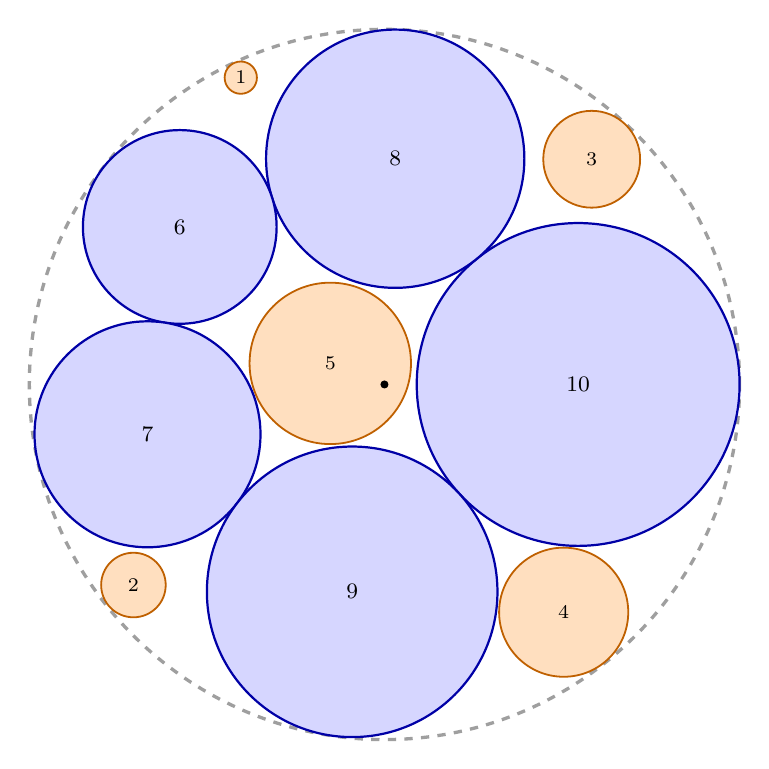
\begin{tikzpicture}[x=.205cm,y=.205cm]
 \draw[gray!75,dashed,very thick] (0,0) circle (22.000193);
 \foreach \x/\y/\rad/\id in
  {-8.901/19.006/1/1,-15.551/-12.425/2/2,12.838/13.952/3/3,11.103/-14.109/4/4,-3.357/1.306/5/5}{
  \draw[fill=orange!25,draw=orange!75!black,line width=.65pt] (\x,\y) circle (\rad);
  \node[font=\scriptsize] at (\x,\y) {$\id$};}
 \foreach \x/\y/\rad/\id in
  {12.00019/0/10/10,0.667074/13.984292/8/8,-12.679903/9.758394/6/6,-14.679116/-3.086961/7/7,-1.999566/-12.845496/9/9}{
  \draw[fill=blue!16,draw=blue!65!black,line width=.8pt] (\x,\y) circle (\rad);
  \node[font=\footnotesize] at (\x,\y) {$\id$};}
 \fill (0,0) circle (.25);
\end{tikzpicture}
\caption{Illustrative optimal ten-disk configuration.  Blue: five mutually
contacting wall disks.  Orange: five rationally placed additional disks.
Neither feasibility nor tangency is inferred from the rounded drawing.}
\label{fig:witness}
\end{figure}

\section{A universal radial cover for the six-disk lower bound}
The lower bound is proved using only disks $5,6,7,8,9,10$; disks $1$--$4$
can be dropped from an impossible-packing argument.  Suppose a ten-disk
packing existed with $R<R_0$.  Then $R<\Rcap$, and for each
$i\in\{5,\ldots,10\}$, containment and separation imply
\begin{equation}\label{eq:init}
\max\left(0,\max_{j\ne i}(i+2j-\Rcap)\right)
 \le s_i\le\Rcap-i,\qquad (j=5,\ldots,10).
\end{equation}
These give strictly positive lower radii for all six selected centers.
We bisect these rational intervals at rational midpoints and propagate
$s_i+s_j\ge i+j$.  Every pair of children covers the parent, so the tree
covers \emph{all} radial vectors of hypothetical packings, not a sample.

The six center directions admit $(6-1)!/2=60$ possible cyclic orders up
to rotation and reflection, rooted at disk $10$.  On each terminal radial
box, rational angle ticks are checked for all $15$ pairs, and
Lemma~\ref{lem:neg} closes every incompatible order unless the main-order
geometric terminal rule below applies.

\begin{lemma}[Wall-angle monotonicity on a certified box]\label{lem:barrier}
Let the projection of the six-disk center order to the five labels
$\{6,7,8,9,10\}$ be exactly $(10,8,6,7,9)$.  Suppose the radial box,
with every selected $s_i$ allowed to increase up to $\Rcap-i$, satisfies
for every consecutive pair $(i,j)$ in this five-cycle
\begin{align*}
 \ell_i+\ell_j&>i+j,\\
 \max\{\lvert\ell_i-(\Rcap-j)\rvert,
         \lvert(\Rcap-i)-\ell_j\rvert\}&<i+j,\\
 \ell_i^2-(\Rcap-j)^2+(i+j)^2&>0,\\
 \ell_j^2-(\Rcap-i)^2+(i+j)^2&>0.
\end{align*}
Then no packing in the box is possible for any $R<R_0$.
\end{lemma}
\begin{proof}
On the indicated rectangles, the necessary angle
\eqref{eq:phi} is in its smooth triangle-inequality domain, and
\[
 \frac{\partial\phi_{ij}}{\partial s_i}
 =-\frac{s_i^2-s_j^2+(i+j)^2}
         {2s_i^2s_j\sin\phi_{ij}}<0,
\]
with the analogous derivative in $s_j$.  Thus replacing the five radial
coordinates, \emph{only in the angle formula}, by their containment maxima
$R-i$ can only decrease the sum of the five required angles.  Therefore
any feasible packing would satisfy
\[
 2\pi\ge\sum_{(i,j)\text{ in five-cycle}}\phi_{ij}(s_i,s_j)
        \ge\mathcal B(R)>\mathcal B(R_0)=2\pi,
\]
where strictness uses $R<R_0$ and the decreasing property of
$\mathcal B$.  This is impossible.  No physical disk movement is asserted.
\end{proof}

\begin{proposition}[Exhaustive rational terminal certificate]\label{prop:tree}
There exists a binary tree of rational radial boxes with the exact
statistics in Table~\ref{tab:tree}.  Every terminal box either excludes
all sixty orders using certified negative cycles, or satisfies the
hypotheses of Lemma~\ref{lem:barrier} for every order not already excluded.
Consequently no disks of radii $5,6,7,8,9,10$ can fit at $R<R_0$.
\end{proposition}
\begin{proof}
The accompanying JSON certificate gives the splitting disk and exact
rational cut at each internal node.  Every terminal node stores rational
angle ticks and one simple negative cycle per excluded linearized order.
The verifier checks every cosine Taylor witness, edge orientation, cycle
closure, and strictly negative exact rational edge sum.  At the other
four terminal nodes it independently checks every inequality of
Lemma~\ref{lem:barrier}, and verifies that any order lacking a negative
cycle has five-disk projection $(10,8,6,7,9)$.  The verifier recursively
reconstructs every box and checks the complete set of sixty orders,
without trusting the discovery program or the proposed classifications.
\end{proof}
\begin{table}[htbp]\centering
\caption{Exact replay of the six-disk lower-bound certificate.}\label{tab:tree}
\begin{tabular}{lr}\toprule
Property & Verified count\\\midrule
Total tree nodes & 75\\
Rational midpoint splits & 37\\
Terminal boxes with all orders excluded by negative cycles & 34\\
Terminal boxes requiring the wall-angle monotonicity rule & 4\\
Unresolved terminal boxes & 0\\
Maximum depth & 30\\\bottomrule
\end{tabular}
\end{table}

\section{Why five largest disks alone do not suffice}
The five disks of radii $6,7,8,9,10$ can in fact fit into a container of
radius $219/10=21.9<R_0$ in a \emph{different} cyclic order.
An exact rational witness, in the order $(10,6,9,8,7)$, is
\[
\begin{aligned}
 p_{10}&=(11.88,0),&p_6&=(5.26,14.983),\\
 p_9&=(-9.029,9.185),&p_8&=(-11.333,-8.013),\\
 p_7&=(2.593,-14.652).&&
\end{aligned}
\]
All containment and ten pairwise separation inequalities for these five
disks hold strictly, as can be checked directly by squaring the rational
coordinates.  This demonstrates why incorporating disk $5$ into the
\emph{lower-bound} case analysis is indispensable to this proof strategy.

\section{Proof of the main theorem and reproducibility}
\begin{proof}[Proof of Theorem~\ref{thm:main}]
Lemma~\ref{lem:root} supplies the exact critical root.  Lemma~\ref{lem:witness}
proves $\Rstar\le R_0$.  Proposition~\ref{prop:tree} excludes even the
six-disk subset of radii $5,\ldots,10$ at every $R<R_0$.  Hence the full
ten-disk packing cannot exist there, proving $\Rstar\ge R_0$.
\end{proof}

The certificate and independent replay components are supplied alongside
this manuscript.  From their common directory run
\begin{quote}\ttfamily\small
python3 certify\_integer\_ten\_global.py
\end{quote}
This invokes \path{verify_ten_upper.py} for the angle root and exact
witness and \path{verify_ten_global_tree.py} for the global finite
cover.  The verifier uses Python integers, \texttt{Fraction}, integer square
roots, and rational Taylor enclosures for trigonometric quantities; candidate
angle ticks may be found using floating point \emph{before} verification.
Optimized Python modes \texttt{-O} and \texttt{-OO} are rejected because the
checkers use \texttt{assert}.  The mathematical soundness claim remains
conditional on the correctness of these programs, the Python runtime and
standard-library semantics, and the certificate files.  It is not an
end-to-end proof-assistant formalization, and has not received independent
peer review.

\begin{thebibliography}{9}
\bibitem{packomania}
E. Specht, \emph{The best known packings of unequal circles with integer
radii in a circle}, Packomania, updated September 10, 2026,
\url{https://packomania.com/ccin/ccin.html}.
\end{thebibliography}
\end{document}
